%% \documentclass{report}
%% \usepackage{fullpage}
%% \usepackage{tikz}
%% \usepackage[utf8]{inputenc}
%% \usepackage[OT1]{fontenc}

%% \begin{document}

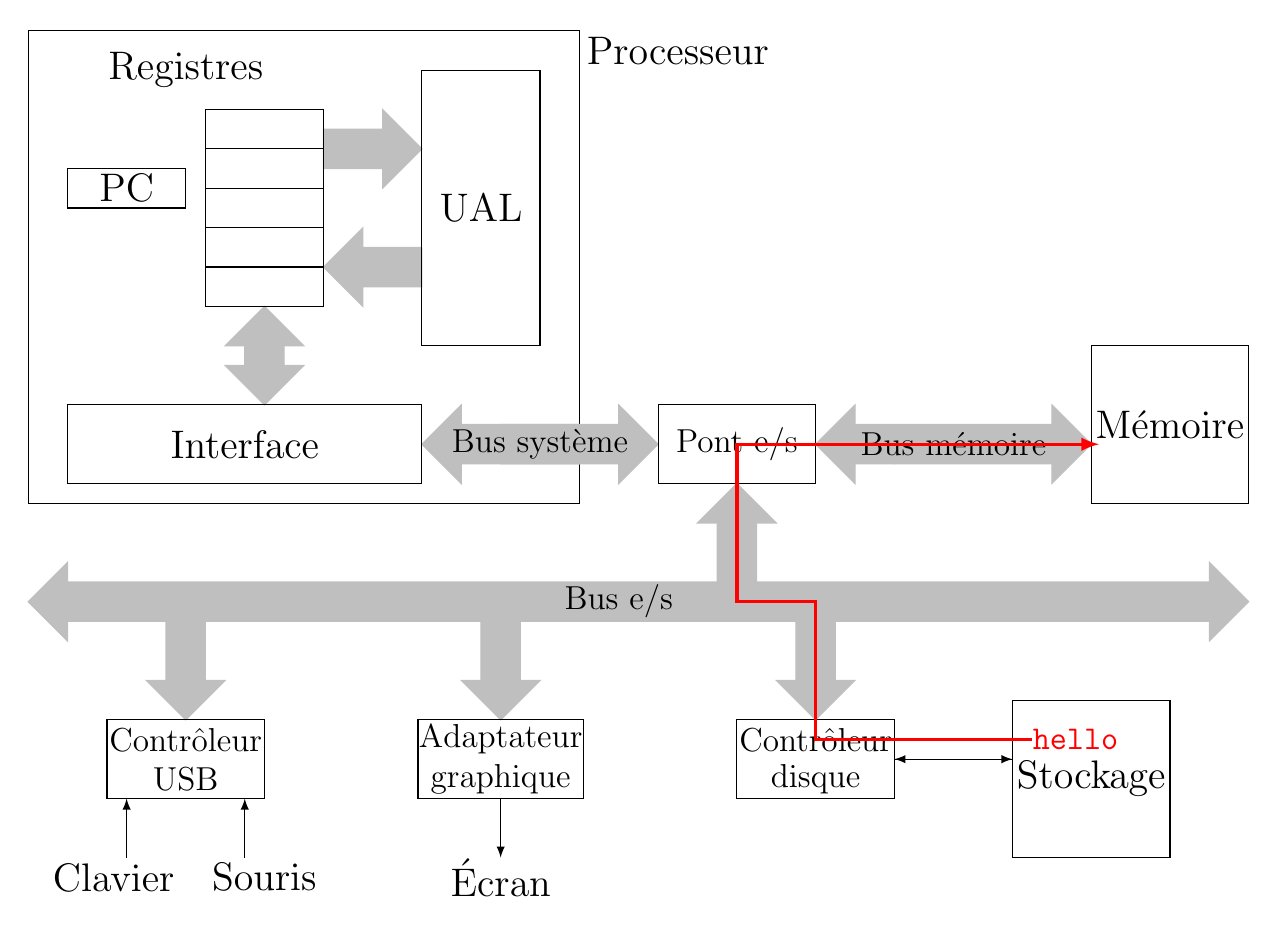
\begin{tikzpicture}

\newcommand{\myarrowright}[3]{% x depart, y depart, longueur
\draw[black!25,fill=black!25] (#1,#2+0.25) -- (#1+#3-0.5,#2+0.25) -- (#1+#3-0.5,#2+0.5) -- (#1+#3,#2) -- (#1+#3-0.5,#2-0.5) -- (#1+#3-0.5,#2-0.25) -- (#1,#2-0.25) -- (#1,#2+0.25);
}
\newcommand{\myarrowleft}[3]{% x depart, y depart, longueur
\draw[black!25,fill=black!25] (#1,#2+0.25) -- (#1-#3+0.5,#2+0.25) -- (#1-#3+0.5,#2+0.5) -- (#1-#3,#2) -- (#1-#3+0.5,#2-0.5) -- (#1-#3+0.5,#2-0.25) -- (#1,#2-0.25) -- (#1,#2+0.25);
}
\newcommand{\myarrowup}[3]{% x depart, y depart, longueur
\draw[black!25,fill=black!25] (#1+0.25,#2) -- (#1+0.25,#2+#3-0.5) -- (#1+0.5,#2+#3-0.5) -- (#1,#2+#3) -- (#1-0.5,#2+#3-0.5) -- (#1-0.25,#2+#3-0.5) -- (#1-0.25,#2) -- (#1+0.25,#2);
}
\newcommand{\myarrowdown}[3]{% x depart, y depart, longueur
\draw[black!25,fill=black!25] (#1+0.25,#2) -- (#1+0.25,#2-#3+0.5) -- (#1+0.5,#2-#3+0.5) -- (#1,#2-#3) -- (#1-0.5,#2-#3+0.5) -- (#1-0.25,#2-#3+0.5) -- (#1-0.25,#2) -- (#1+0.25,#2);
}


%% \foreach \i in {0,...,15} {
%%   \foreach \j in {-20,...,0} {
%%     \node[black!25] at (\i,\j) {\i,\j};
%%   }
%% }

%cpu
\draw (0,0) rectangle (7,-6);
\node at (8.25,-0.25) {\Large Processeur};
%bus registers->ALU
\myarrowright{3.75}{-1.5}{1.25}
%bus ALU->registers
\myarrowleft{5}{-3}{1.25}
%bus CPU->i/o bridge
\myarrowright{6}{-5.25}{2}
%bus i/o bridge->CPU
\myarrowleft{7}{-5.25}{2}
%bus i/o brige->memory
\myarrowright{11}{-5.25}{2.5}
%bus memory->i/o bridge
\myarrowleft{11}{-5.25}{1}
%i/o bus->i/o bridge
\myarrowup{9}{-7}{1.25}
%bus interface->registers
\myarrowup{3}{-4}{0.5}
%registers->bus interface
\myarrowdown{3}{-4}{0.75}
%i/o bus->usb controller
\myarrowdown{2}{-7.25}{1.5}
%i/o bus->graphics adapter
\myarrowdown{6}{-7.25}{1.5}
%i/o bus->disk controller
\myarrowdown{10}{-7.25}{1.5}
%pc
\draw (0.5,-1.75) rectangle (2,-2.25);
\node at (1.25,-2) {\Large PC};
%other registers
\draw (2.25,-1) rectangle (3.75,-3.5);
\draw (2.25,-1.5) -- (3.75,-1.5);
\draw (2.25,-2) -- (3.75,-2);
\draw (2.25,-2.5) -- (3.75,-2.5);
\draw (2.25,-3) -- (3.75,-3);
\node at (2,-0.5) {\Large Registres};
%alu
\draw (5,-0.5) rectangle (6.5,-4);
\node at (5.75,-2.25) {\Large UAL};
%bus interface
\draw (0.5,-4.75) rectangle (5,-5.75);
\node at (2.75,-5.25) {\Large Interface};
%i/o bridge
\draw (8,-4.75) rectangle (10,-5.75);
\node at (9,-5.25) {\large Pont e/s};
%memory
\draw (13.5,-4) rectangle (15.5,-6);
\node at (14.5,-5) {\Large Mémoire};
%i/o bus
\myarrowleft{8}{-7.25}{8}
\myarrowright{8}{-7.25}{7.5}
%usb controller
\draw (1,-8.75) rectangle (3,-9.75);
\node at (2,-9) {\large Contrôleur};
\node at (2,-9.5) {\large USB};
\draw[-latex] (1.25,-10.5) -- (1.25,-9.75);
\node at (1.25,-10.75) {\Large Clavier~~~};
\draw[-latex] (2.75,-10.5) -- (2.75,-9.75);
\node at (2.75,-10.75) {\Large ~~~Souris};
%graphics adapter
\draw (4.95,-8.75) rectangle (7.05,-9.75);
\node at (6,-9) {\large Adaptateur};
\node at (6,-9.5) {\large graphique};
\draw[-latex] (6,-9.75) -- (6,-10.5);
\node at (6,-10.75) {\Large Écran};
%disk controller
\draw (9,-8.75) rectangle (11,-9.75);
\node at (10,-9) {\large Contrôleur};
\node at (10,-9.5) {\large disque};
\draw[-latex] (11,-9.25) -- (12.5,-9.25);
\draw[-latex] (12.5,-9.25) -- (11,-9.25);
%disk
\draw (12.5,-8.5) rectangle (14.5,-10.5);
\node at (13.5,-9.5) {\Large Stockage};
%bus names
\node at (7.5,-7.25) {\large Bus e/s};
\node at (11.75,-5.25) {\large Bus mémoire};
\node at (6.5,-5.25) {\large Bus système};


\draw[red,very thick,-latex] (12.75,-9) -- (10,-9) -- (10,-7.25) -- (9,-7.25) -- (9,-5.25) -- (13.6,-5.25);
\node[red] at (13.3,-9) {\large \tt hello};

\end{tikzpicture}

%\end{document}
